% print in Okular with kop21_neu3 (Options -> Duplex Printing -> Long side)

% leaflet document class
\documentclass[
  % don't rotate back page while writing the flyer
  %notumble,
  % disable pre-set fold mark
  nofoldmark,
  % use portrait format
  portrait,
  % font size
  12pt,
]{leaflet}

% language and encodings
\usepackage[ngerman,american]{babel}

% amsmath with improvements
\usepackage{mathtools}

% use GoMono as typewriter font
\usepackage[
  % otherwise, bold is not available ("undefined font shape" warnings)
  type1,
  % scale to match main font size
  scale=0.88,
]{GoMono}

% use TeX Gyre Heros as sans-serif font
\usepackage{tgheros}

% need T1 font encoding for Charter,
% otherwise there will be "undefined font shape" warnings
\usepackage[T1]{fontenc}

% use Bitstream Charter as main font
\usepackage[bitstream-charter]{mathdesign}

% micro-typographic adjustments
\usepackage[
  % don't deactivate extensions due to document class draft option
  final,
  % increase letter spacing in small-caps
  tracking=smallcaps,
  % font expansion: don't stretch/shrink lines by more than 1%,
  % default of 2% looks a bit weird
  stretch=10,
  shrink=10,
]{microtype}

% consistent style of units and numbers
\usepackage{siunitx}

% TikZ
\usepackage{tikz}

% insert space if needed
\usepackage{xspace}

% string functions
\usepackage{xstring}

% hyperlinks
\usepackage{hyperref}

% automatically replace "l" with \ell in math mode
\makeatletter
  \mathcode`l="8000
  \begingroup
    \lccode`\~=`\l
    \DeclareMathSymbol{\lsb@l}{\mathalpha}{letters}{`l}
    \lowercase{\gdef~{\ifnum\the\mathgroup=\m@ne \ell \else \lsb@l \fi}}%
  \endgroup
\makeatother

% set front and back page
\AddToBackground{1}{\includegraphics[height=\paperheight]{front}}
%\AddToBackground{4}{\includegraphics[height=\paperheight]{back}}

% define line colors (mix between MATLAB and matplotlib colors)
\definecolor{C0}{rgb}{0.000,0.447,0.741}
\definecolor{C1}{rgb}{0.850,0.325,0.098}
\definecolor{C2}{rgb}{0.749,0.561,0.102}
\definecolor{C3}{rgb}{0.494,0.184,0.556}
\definecolor{C4}{rgb}{0.466,0.674,0.188}
\definecolor{C5}{rgb}{0.301,0.745,0.933}
\definecolor{C6}{rgb}{0.635,0.078,0.184}
\definecolor{C7}{rgb}{0.887,0.465,0.758}
\definecolor{C8}{rgb}{0.496,0.496,0.496}

% define university CD colors
\definecolor{anthrazit}{RGB}{62,68,76}
\definecolor{mittelblau}{RGB}{0,81,158}
\definecolor{hellblau}{RGB}{0,190,255}

% set up hyperref
\hypersetup{
  % set metadata
  pdftitle={%
    B-Splines for Sparse Grids:
    Algorithms and Application to Higher-Dimensional Optimization%
  },
  pdfauthor={Julian Valentin},
  pdfcreator={LaTeX, hyperref},
  % underline links instead of putting a framed box around them
  pdfborderstyle={/S/U/W 1},
  % set link colors
  citebordercolor=C1,
  filebordercolor=C1,
  linkbordercolor=C1,
  menubordercolor=C1,
  runbordercolor=C1,
  urlbordercolor=C0,
}

% don't justify text
\raggedright

% decrease top and bottom margins from 11mm to 8mm
\setmargins{8mm}{8mm}{8mm}{8mm}

% TikZ libraries
\usetikzlibrary{
  % coordinate calculations
  calc,
}

% excerpt from thesis as rotated circle, arguments:
% {x coordinate on flyer}{y coordinate on flyer}{radius on flyer}
% {x coordinate on page}{y coordinate on page}{radius on page}{page no.}
\newcommand*{\thesisCircle}[7]{
  %\fill[black,opacity=0.4] ($({#1+1mm},{#2-1mm})$) circle (#3+0.5mm);
  \node[thesis circle={#3}{#4}{#5}{#6}{#7}] at (#1,#2) {};
}
\newlength{\tcleft}
\newlength{\tcbottom}
\newlength{\tcright}
\newlength{\tctop}
\newlength{\tcwidth}
\newcommand*{\tcangcon}{0}
\tikzset{
  thesis circle/.style n args={5}{
    circle,
    anchor=center,
    draw=mittelblau,
    fill=mittelblau!20,
    minimum size=2*#1,
    inner sep=0mm,
    line width=0.4mm,
    path picture={
      \node[anchor=center,rotate=\tcangcon] at (0,0) {%
        \def\tcpage{\numexpr#5+2\relax}%
        \pgfmathsetlength{\tcleft}{#2-#4}%
        \pgfmathsetlength{\tcbottom}{297mm-(#3+#4)}%
        \pgfmathsetlength{\tcright}{210mm-(#2+#4)}%
        \pgfmathsetlength{\tctop}{#3-#4}%
        \pgfmathsetlength{\tcwidth}{2*#1}%
        \includegraphics[
          page=\tcpage,
          trim={\tcleft{} \tcbottom{} \tcright{} \tctop{}},
          clip,
          width=\tcwidth,
        ]{thesis}%
      };
    }
  }
}

% define macros
\newcommand*{\abs}[1]{|#1|}
\newcommand*{\basis}[1]{\varphi_{#1}}
\newcommand*{\bspl}[2]{\varphi^{#1}_{#2}}
\newcommand*{\cardbspl}[1]{b^{#1}}
\newcommand*{\ceq}{\coloneqq}
\newcommand*{\charfun}[1]{\chi_{#1}}
\newcommand*{\containsvector}[3]{%
  \protect\IfSubStr{\detokenize{#1}}{\detokenize{\*}}{#2}{#3}%
}
\newcommand*{\Cp}[1]{\mathcal{C}^{#1}}
\newcommand*{\follows}{\ensuremath{\rightsquigarrow}\xspace}
\newcommand*{\gp}[1]{\containsvector{#1}{\*x}{x}_{#1}}
\newcommand*{\hopint}[1]{\mathopen[#1\mathclose[}
\newcommand*{\ifnotempty}[2]{\if\relax\detokenize{#1}\relax\else#2\fi}
\newcommand*{\landauO}[1]{\mathcal{O}(#1)}
\newcommand*{\linop}{\mathfrak{L}}
\newcommand*{\linopinv}{\mathfrak{L}^{-1}}
\newcommand*{\Ltwo}{L^2}
\newcommand*{\ngp}{N}
\newcommand*{\norm}[2][]{\lVert#2\rVert_{#1}}
\newcommand*{\normone}[1]{\norm[1]{#1}}
\newcommand*{\objfun}{f}
\newcommand*{\sgintp}{f^\sparse}
\newcommand*{\sparse}{\mathrm{s}}
\newcommand*{\surplus}[1]{\alpha_{#1}}
\renewcommand*{\vec}[1]{{\boldsymbol{#1}}}
\def\*#1{\vec{#1}}
\newcommand*{\vlinin}[1][]{\*u\ifnotempty{#1}{^{#1}}}
\newcommand*{\vlinout}[1][]{\*y\ifnotempty{#1}{^{#1}}}

\begin{document}
  \null\clearpage
  
  
  
  \hfill{}1\vspace{-3.7em}
  
  \section{Sparse Grids}
  
  \paragraph{Motivation}
  
  Inverse problems\\
  \follows Expensive objective functions (simulations)\\
  \follows Construct surrogates by interpolation:\\
  $
    \objfun \approx \sgintp
    \ceq \sum_{\*l,\*i} \surplus{\*l,\*i} \basis{\*l,\*i}
  $,\;\;
  $\objfun(\gp{\*l,\*i}) = \sgintp(\gp{\*l,\*i})$;\\
  Full grids suffer from curse of dimensionality
  
  \vspace{0.5em}\hfill
  \tikz{\thesisCircle{0mm}{0mm}{15mm}{70mm}{80mm}{45mm}{37}}
  
  \vspace{-2.5em}
  \vspace{-30mm}
  
  \paragraph{Construction}
  
  Nodal to hier-\\
  archical basis
  \follows Order basis\\
  functions by level $\*l$
  \follows $\basis{\*l,\*i}$\\
  with large $\normone{\*l}$ unimportant\\
  \follows A priori selection of $\basis{\*l,\*i}$\\
  and $\gp{\*l,\*i}$ such that $\Ltwo$ error de-\\
  teriorates only slightly, no curse
  
  \vspace{-1em}
  
  \paragraph{Spatial adaptivity}
  
  Use hierarchical surpluses $\abs{\surplus{\*l,\*i}}$
  to identify key regions with oscillations\\
  \follows Insert children grid points a posteriori
  
  \section{Hierarchical B-Splines}
  
  \paragraph{Motivation}
  
  Most hierarchical bases (e.g., hat functions)
  not continuously differentiable\\
  \follows Gradient-based optimization difficult
  
  \vspace{0.5em}
  \tikz{\thesisCircle{0mm}{0mm}{15mm}{150.5mm}{100.5mm}{25mm}{52}}
  
  \vspace{-2.5em}
  \vspace{-30mm}
  
  \paragraph{\hspace{29mm}Definition}
  
  B-spline $\cardbspl{p}$ of\\\hspace{31mm}
  degree $p$ is $(p+1)$-times\\\hspace{32mm}
  convolution of $\cardbspl{0} \ceq \charfun{\hopint{0, 1}}$\\\hspace{32mm}
  with itself; Cox--de Boor\\\hspace{31mm}
  recursion formula as\\\hspace{28mm}
  alternative
  
  \vspace{-1em}
  
  \paragraph{Advantages}
  
  Generalize hat functions;
  compactly supported;
  basis of spline space;
  higher order of convergence;
  additional parameter $p$;
  $\Cp{p-1}$-smoothness;
  flexibility;
  many nice numerical/algorithmic properties
  
  \clearpage
  
  
  
  \hfill{}2\vspace{-3.7em}
  
  \section{Results in Theory/Algorithms}
  
  \paragraph{Mathematical framework}
  
  Sparse grid framework with general tensor product basis functions;
  all algorithms are rigorously proven using invariants;
  most bases can be combined
  (modified, Clenshaw--Curtis, not-a-knot, (weakly) fundamental)
  
  \vspace{0.5em}\hfill
  \tikz{\thesisCircle{0mm}{0mm}{15mm}{144mm}{102mm}{25mm}{67}}
  
  \vspace{-2.5em}
  \vspace{-30mm}
  
  \paragraph{Boundary conditions}
  
  Appli-\\
  cation of not-a-knot bound-\\
  ary conditions to hierarchi-\\
  cal B-splines to replicate po-\\
  lynomials and achieve opti-\\
  mal convergence order $p+1$
  
  \vspace{-1em}
  
  \paragraph{Sparse grid algorithms}
  
  Linear operators $\vlinout = \linop[\vlinin]$,
  hierarchization as example:
  Given $\objfun(\gp{\*l,\*i})$,
  find $\surplus{\*l,\*i}$ such that
  $\objfun(\gp{\*l,\*i}) = \sgintp(\gp{\*l,\*i})$;
  high complexity $\landauO{N^2 (N+d)}$ (linear system)
  
  \vspace{0.5em}
  \tikz{\thesisCircle{0mm}{0mm}{15mm}{50mm}{105mm}{30mm}{89}}
  
  \vspace{-2.5em}
  \vspace{-30mm}
  
  \paragraph{\hspace{29mm}Dimensionally adaptive grids\hspace{-5mm}}
  
  \hspace*{31mm}
  Combinatorial proof of\\\hspace{32mm}
  combination technique; new\\\hspace{32mm}
  method of residual interpo-\\\hspace{31mm}
  lation operating on active\\\hspace{28mm}
  hierarchical subspaces
  
  \vspace{0.5em}\hfill
  \tikz{\thesisCircle{0mm}{0mm}{15mm}{51mm}{64mm}{26mm}{115}}
  
  \vspace{-2.5em}
  \vspace{-30mm}
  
  \paragraph{Spatially adaptive grids}
  
  \ \\
  Breadth-first search for fun-\\
  damental splines requires\\
  $\landauO{\ngp^2 d}$ complexity ($\ngp$ grid\\
  points, $d$ dimensions); alter-\\
  natively $\landauO{\ngp d}$ with unidirec-\\
  tional principle if chain points for\\
  $\linopinv$ exist;
  weakly fundamental splines minimize number of points and
  enable Hermite hierarchization
  
  \clearpage
  
  
  
  \vspace*{\fill}
  
  \rlap{%
    \hspace{2mm}%
    \begin{tikzpicture}
      \thesisCircle{31.6mm}{192.3mm}{22.0mm} {80mm} {80mm}{45mm}{124}
      \thesisCircle{10.0mm}{159.5mm}{17.0mm}{140mm}{130mm}{30mm}{100}
      \thesisCircle{45.7mm}{153.5mm}{19.0mm}{140mm}{140mm}{25mm}{132}
      \thesisCircle{20.0mm}{122.1mm}{21.5mm}{120mm}{150mm}{40mm} {50}
      \thesisCircle{58.5mm}{119.4mm}{17.0mm} {50mm}{100mm}{30mm}{236}
      \thesisCircle{41.6mm} {86.2mm}{20.0mm} {70mm}{200mm}{30mm}{149}
      \thesisCircle {7.5mm} {88.5mm}{14.0mm}{125mm}{108mm}{26mm}{161}
      \thesisCircle{16.6mm} {58.5mm}{17.0mm}{140mm} {65mm}{30mm}{199}
      \thesisCircle{50.4mm} {48.9mm}{18.0mm}{152mm} {70mm}{30mm}{109}
    \end{tikzpicture}%
  }
  
  \vspace*{\fill}
  
  \clearpage
  
  
  
  \hfill{}3\vspace{-3.7em}
  
  \section{Results in Applications}
  
  \paragraph{Optimization of test functions}
  
  Unconstrained and constrained test problems;
  optimization gaps up to six orders of magni-\\tude
  smaller for cubic B-splines than for hat functions
  
  \vspace{0.5em}
  \tikz{\thesisCircle{0mm}{0mm}{15mm}{100mm}{90mm}{40mm}{146}}
  
  \vspace{-2.5em}
  \vspace{-30mm}
  
  \paragraph{\hspace{29mm}Fuzzy extension principle}
  
  \hspace*{31mm}
  Propagation of fuzzy uncer-\\\hspace{32mm}
  tainties from input to output\\\hspace{32mm}
  of a model; generation of\\\hspace{31mm}
  spatially adaptive sparse\\\hspace{28mm}
  grids via problem-tailored\\\hspace{25mm}
  fuzzy Novak--Ritter criterion
  
  \vspace{0.5em}\hfill
  \tikz{\thesisCircle{0mm}{0mm}{15mm}{140mm}{80mm}{35mm}{247}}
  
  \vspace{-2.5em}
  \vspace{-30mm}
  
  \paragraph{Topology optimization}
  
  Cho-\\
  lesky factor interpolation to\\
  preserve positive definite-\\
  ness and explicit continuous\\
  derivatives of elasticity ten-\\
  sors;
  3D problems with \num{40000}\\shape variables
  
  \vspace{0.5em}
  \tikz{\thesisCircle{0mm}{0mm}{15mm}{110mm}{65mm}{26mm}{176}}
  
  \vspace{-2.5em}
  \vspace{-30mm}
  
  \paragraph{\hspace{29mm}Biomechanics}
  
  Reduce com-\\\hspace{31mm}
  putational time by up to\\\hspace{32mm}
  \SI{99}{\percent} by using B-spline sur-\\\hspace{32mm}
  rogates on sparse grids in-\\\hspace{31mm}
  stead of complex continuum-\\\hspace{28mm}
  mechanical model of human\\\hspace{25mm}
  upper limb
  
  \vspace{0.5em}\hfill
  \tikz{\thesisCircle{0mm}{0mm}{15mm}{155mm}{72mm}{25mm}{214}}
  
  \vspace{-2.5em}
  \vspace{-30mm}
  
  \paragraph{Financial application}
  
  Solve\\
  dynamic portfolio choice\\
  problems of five state vari-\\
  ables and eleven policy vari-\\
  ables via dynamic program-\\
  ming with B-spline surrogates
  
  \clearpage
  
  
  
  \hfill{}4\vspace{-3.7em}
  
  \section{Recommendations/Limitations}
  
  \begin{itemize}
    \item
    You must be able to sample $\objfun$ at arbitrary points;
    scattered point data do not suffice
    
    \item
    $\objfun$ should be defined on a hyper-rectangle
    $[a_1, b_1] \times \dotsb \times [a_d, b_d]$
    
    \item
    Dimensionality $d$ should not be too large (e.g., $d \le 10$)
    
    \item
    $\objfun$ should be ``as smooth as possible''
    (at least as smooth as the basis functions)
  \end{itemize}
  
  \section{Future Work}
  
  Better refinement criteria;
  incorporate con-\\straints if available;
  investigate other applica-\\tions for example
  with dimensional adaptivity;
  use new bases and algorithms for density esti-\\mation and regression;
  true $h$-$p$-adaptivity be-\\yond choosing different degrees
  for different dimensions; \dots
  
  \vfill
  
  \hrule
  
  \paragraph{Literature}
  
  See \href{%
    https://bsplines.org/~valentjn%
  }{%
    \texttt{bsplines.org/\textasciitilde{}valentjn}%
  }
  
  \vspace{-1em}
  
  \paragraph{Software}
  
  SG\textsuperscript{++}
  (\href{https://github.com/SGpp}{\texttt{github.com/SGpp}})
  
  \vspace{-1em}
  
  \paragraph{Acknowledgments}
  
  Thanks to
  D.~Hübner,
  D.~Pflüger,
  P\hspace{-0.1em}.~Schober,
  M.~Sprenger,
  S.~Zimmer,
  and many more.
  
  \vspace{0.5em}
  
  {%
    \footnotesize
    V\hspace{-0.1em}.i.S.d.P\hspace{-0.1em}.\ Julian Valentin,
    Universitätsstr.\ 38, 70569 Stutt-\\gart;
    not an official publication of the Univ.\ of Stuttgart.%
  }
\end{document}
